\chapter{Materialeigenschaften}

\begin{figure}[h]
	\centering
	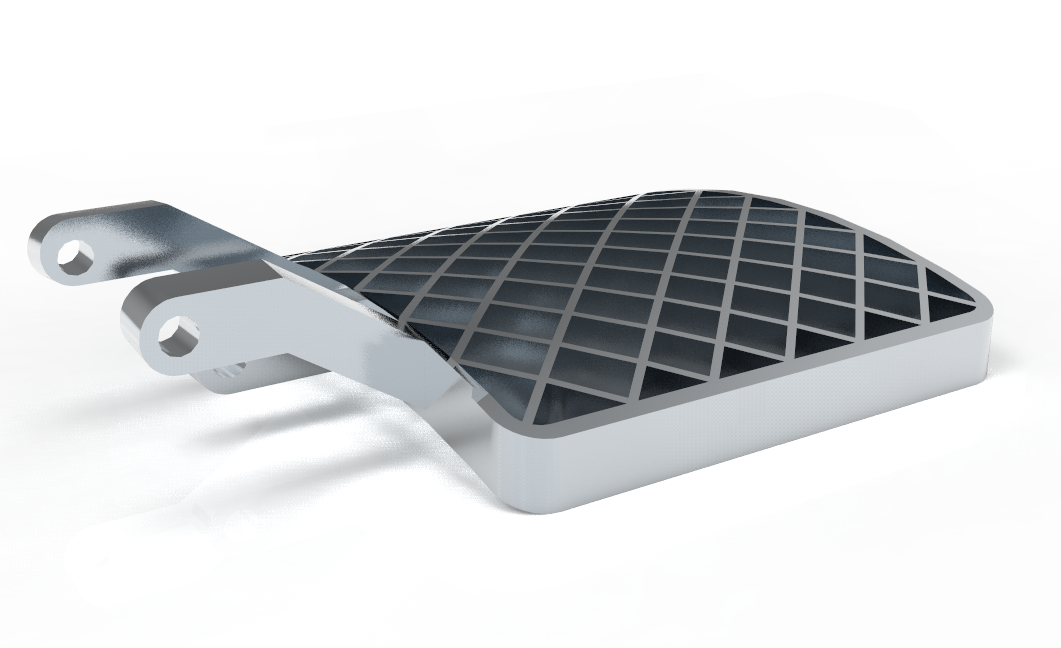
\includegraphics[width=0.5\textwidth]{PreisModell.png}
	\caption{Modell zur Ermitllung der Materialkosten}
	\label{abb_100mmModel}
\end{figure}
\begin{itemize}
		\item $V = 99,70\mathrm{mm}^3$
		\item Benötigter Bauraum: 187,76 x 132,28 x 44,21 mm$^3$
		\item $b = h = 132,28$mm
		\item $s = 14,17$mm
		\item $d_R = 3,78$mm
		\item $d_G = 1,89$mm
		\item Krümmungsradius $=200,21$mm
\end{itemize}
\begin{landscape}
\begin{table}[h]
	\centering
	\begin{tabular}{|c|c|c|c|c|c|c|c|c|}
		\hline
		Werkstoff&Bezeichnung&$\rho$/$\frac{\mathrm{g}}{\mathrm{cm}^3}$&$R_{p,0.2}$/MPa&$R_{p,0.2}$/MPa&$R_\mathrm{spez.}$/$\frac{\mathrm{Nm}}{\mathrm{g}}$&Preis/€&$T_\mathrm{E, max}$/$^\circ$C&$T_\mathrm{Schmelz}$/$^\circ$C\\
		&&&unbehandelt&wärmebehandelt&&&&\\
		\hline \hline
		Aluminium&AlSi10Mg&2,57&230-270&&89,5&1.508,93&530&557\\
		Aluminium&AlSi7Mg0.6&2,67&250-255&&93,6&&&557\\
		\hline
		Edelstahl&1.4404&7,97&480-540&&60,2&4.991,35&850 (w)&1400\\
		Edelstahl&1.4542&7,79&861-861&1262-1262&110,5&2.559,27&550&1400\\
		Edelstahl&"CX"&7,69&840-8400&1650-1670&109,2&&&\\
		Edelstahl&1.4540&7,7&930-1025&1200-1250&120,8&&&\\
		\hline
		Inconel&IN 625&8,15&630-720&640-680&77,3&&950 (w)&1350\\
		Inconel&IN 718&8,15&&1140-1245&140,5&2.597,71&700&1260\\
		Inconel&IN 939&8,15&&1100-1130&135,0&&850&\\
		Inconel&"HX"&8,2&545-630&1200-1200&66,5&&&1355\\
		\hline
		Titan&Ti6Al4V&4,41&1120-1140&&254,0&3.085,12&>700 (w)&1630\\
		Titan&Ti6Al4V Grade 5&4,4&&970-1010&220,5&&870&1604\\
		Titan&Ti6Al4V ELI&4,41&&945-965&214,3&&982&2800\\
		\hline
	\end{tabular}
	\begin{flushright}
		\flushbottom{Quellen: \cite{eos, preise, T1.1, T1.3, T1.4, T2.1, T2.2, T2.3, T2.4, T3.1, T3.2, T3.3, T3.4, T3.5, T3.6, T3.7, T3.8}}
	\end{flushright}
	\caption{Vergleichsdaten der unterschiedlichen Werkstoffe}
	\label{tab_Werkstoffe} 
\end{table}
(w) = Temperatur für Warmumformung
\end{landscape}